\chapter{Implementación de la aplicación}
\label{chap:appvalidation}

\section{Primera iteración}

\subsection{Alcance de la iteración}

En esta primera iteración se van a desarrollar los siguientes requisitos: RF1, RF2, RF3, RF4, RF5, RF6, RF7, RF8, RF9, RF12, RF13, RF14, RF15, RF16, RF17, RF18. 

Además, deberá de crear la base de datos en Supabase, el proyecto en Flutter y conectarlos entre sí. 

Para la autenticación  (login / logout), se va a utilizar el sistema de autenticación de Supabase de correo electrónico y contraseña. Para evitar que cualquier persona pueda crearse una cuenta, las credeciales las proporcionará el desarrollador al usuario. Esto permite controlar el acceso al sistema y, con ello, mejorar la seguridad de la información. 

Para la gestión de clientes y artículos, se crearán las tablas convenientes. 

\subsection{Implementación}

La implementación se ha llevado a cabo en relación a los diseños de los bocetos iniciales del capítulo anterior. Además, se han añadido pantallas de categorías de artículos para permitir una mejor organización de los artículos de la tienda. Tras completar la implementación, hemos obtenido las siguientes pantallas: 

\subsubsection{Pantalla de login}

\begin{figure}[H]
	\centering
	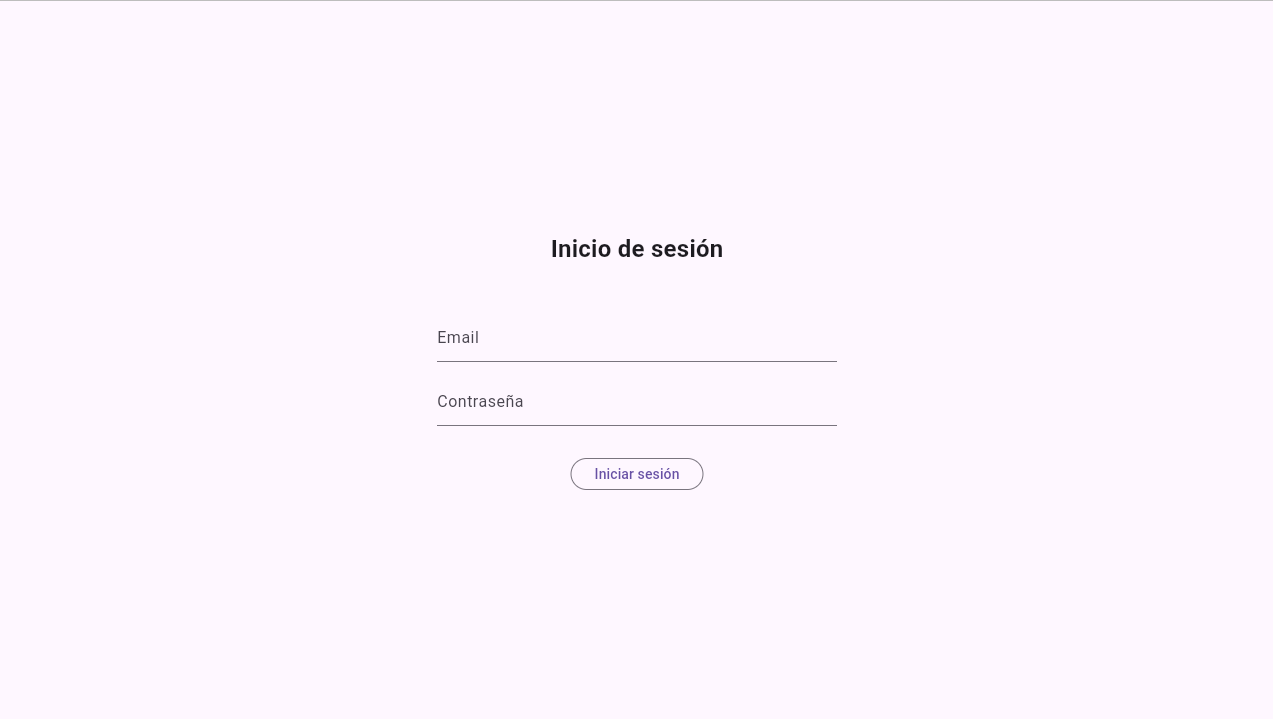
\includegraphics[width=0.7\textwidth]{imagenes/PrimeraIteracion/inicioSesion.png}
	\caption{Interfaz de usuario de inicio de sesión.}
	\label{fig:appInicioSesion}
\end{figure}

\subsubsection{Pantalla de principal}

\begin{figure}[H]
	\centering
	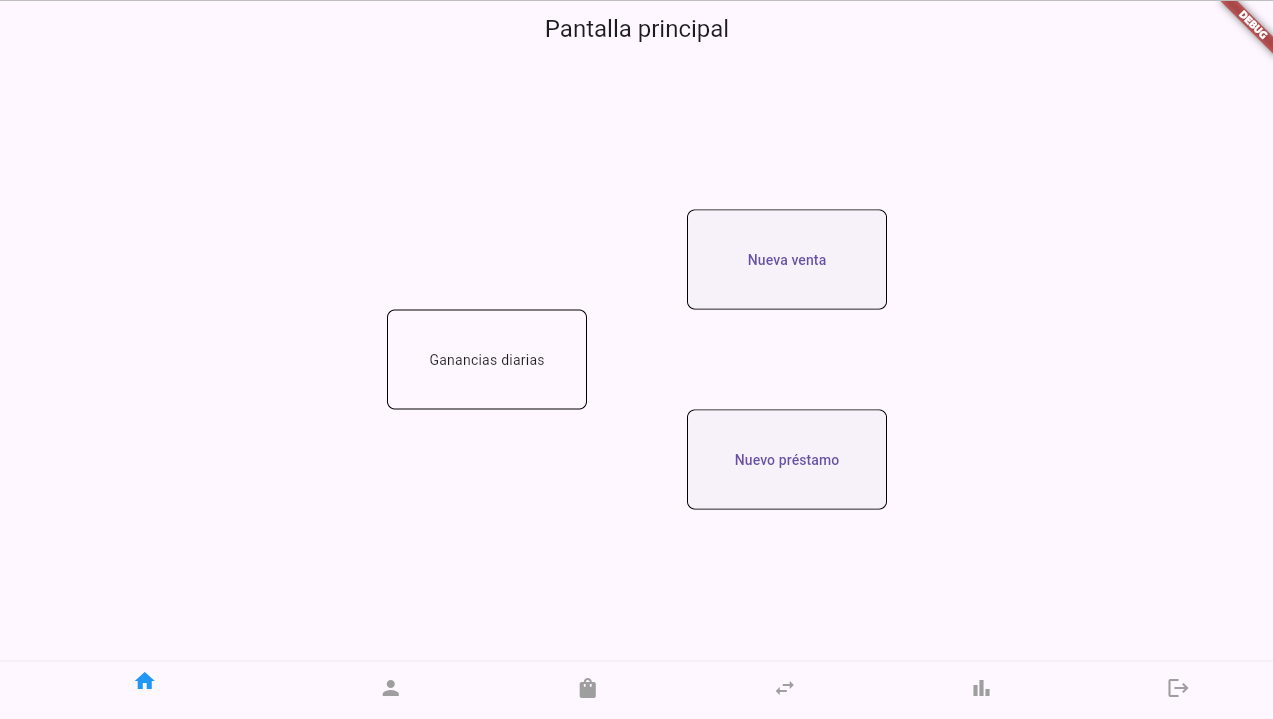
\includegraphics[width=0.7\textwidth]{imagenes/PrimeraIteracion/pantallaPrincipal.png}
	\caption{Interfaz de usuario de la pantalla principal.}
	\label{fig:appPantallaPrincipal}
\end{figure}

\subsubsection{Pantalla de visualización de clientes}

En esta pantalla se verán todos los clientes registrados en la tienda. Se pueden buscar por nombre o filtrar aquellos que deban dinero a la tienda. 

Los clientes que están en positivo en la tienda, es decir, tienen dinero a favor, se muestran con un fondo verde. Los clientes que están en negativo, se muestran con un fondo rojo. Si no tiene dinero a favor ni a deber, se muestran en blanco. 

\begin{figure}[H]
	\centering
	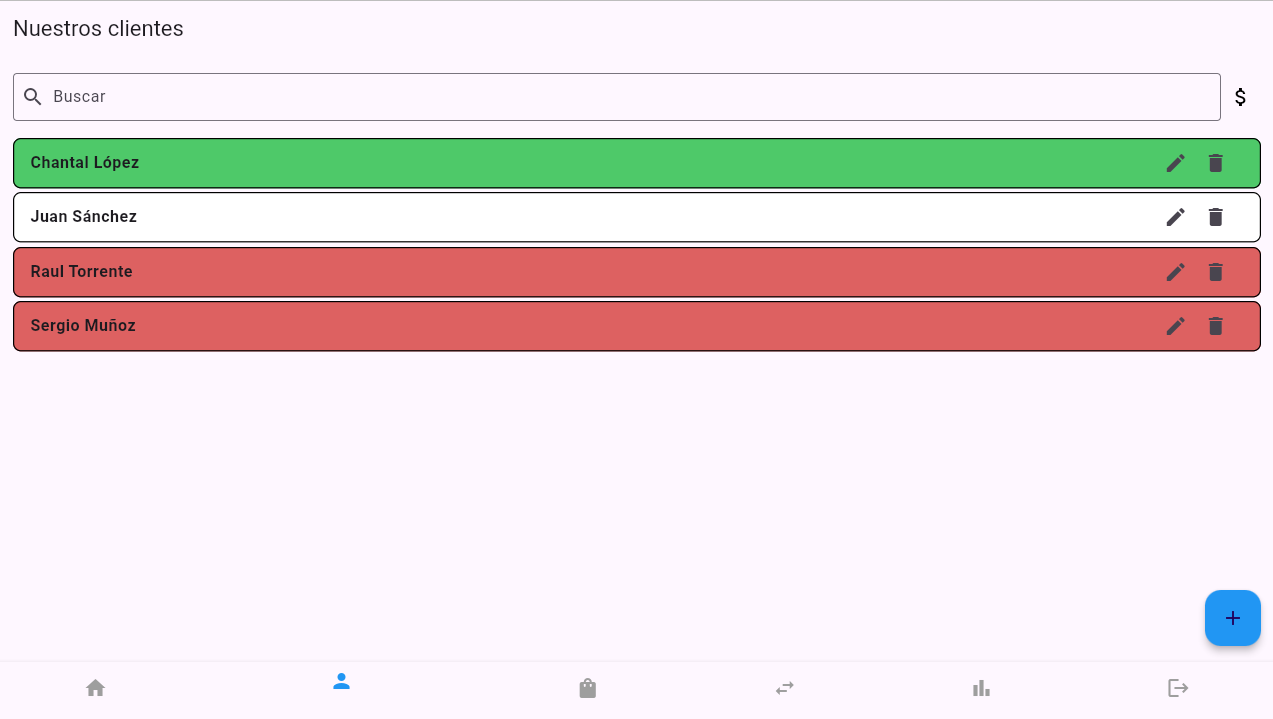
\includegraphics[width=0.7\textwidth]{imagenes/PrimeraIteracion/visualizacionClientes.png}
	\caption{Interfaz de usuario de la pantalla de visualización de clientes.}
	\label{fig:appVisualizarClientes}
\end{figure}

\subsubsection{Pantalla de añadir nuevo cliente}

\begin{figure}[H]
	\centering
	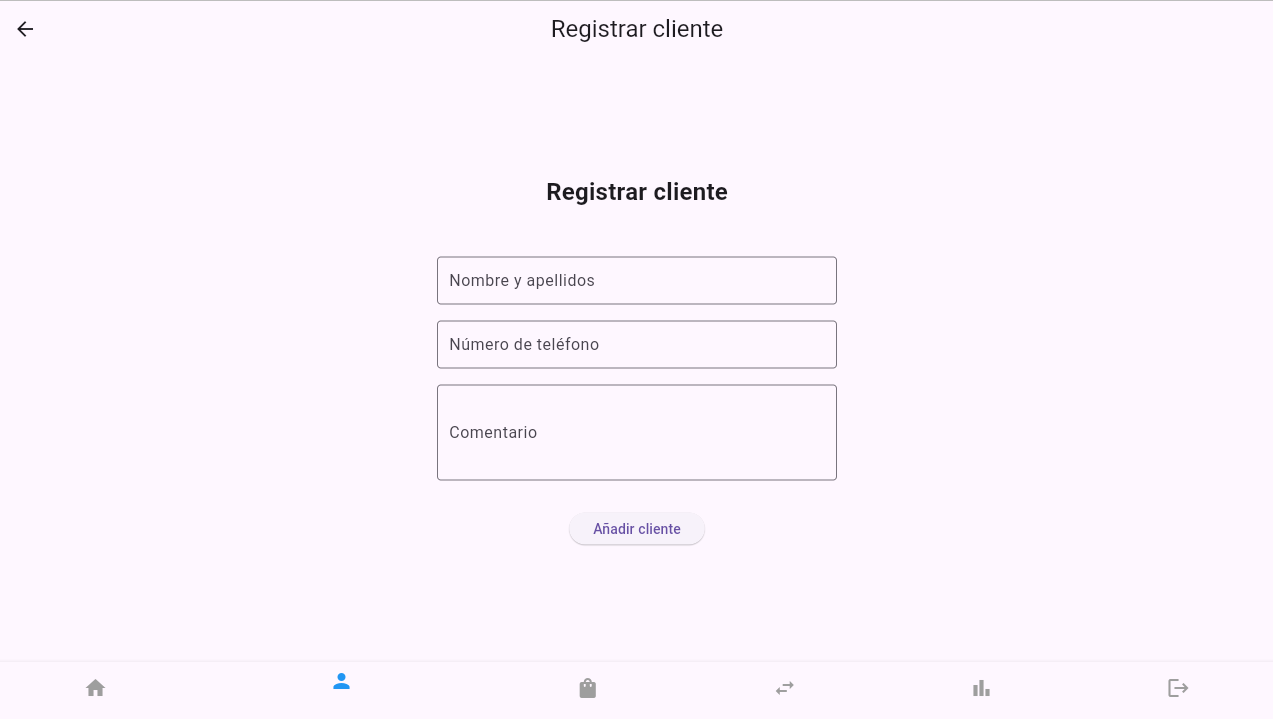
\includegraphics[width=0.7\textwidth]{imagenes/PrimeraIteracion/nuevoCliente.png}
	\caption{Interfaz de usuario de la pantalla de nuevo cliente.}
	\label{fig:appNuevoCliente}
\end{figure}

\subsubsection{Pantalla de editar un cliente existente}

\begin{figure}[H]
	\centering
	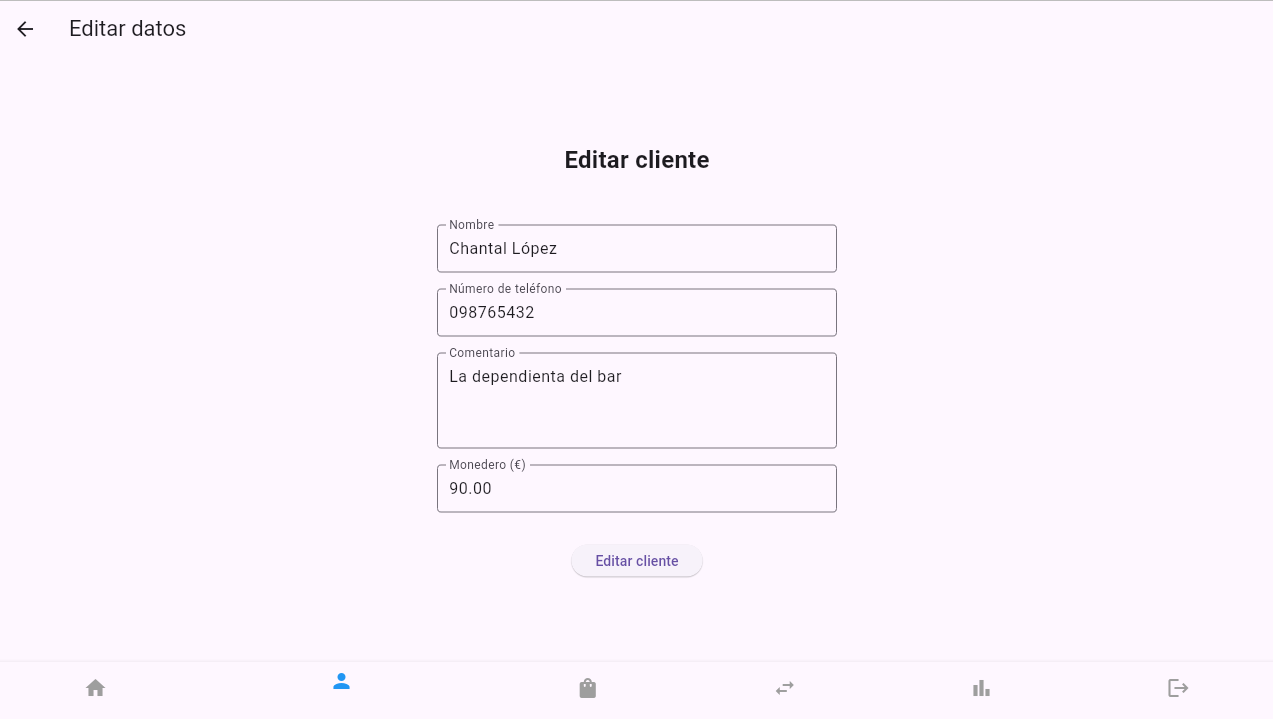
\includegraphics[width=0.7\textwidth]{imagenes/PrimeraIteracion/editarCliente.png}
	\caption{Interfaz de usuario de la pantalla de editar cliente.}
	\label{fig:appEditarCliente}
\end{figure}

\subsubsection{Pantalla de visualizar los datos de un cliente}

\begin{figure}[H]
	\centering
	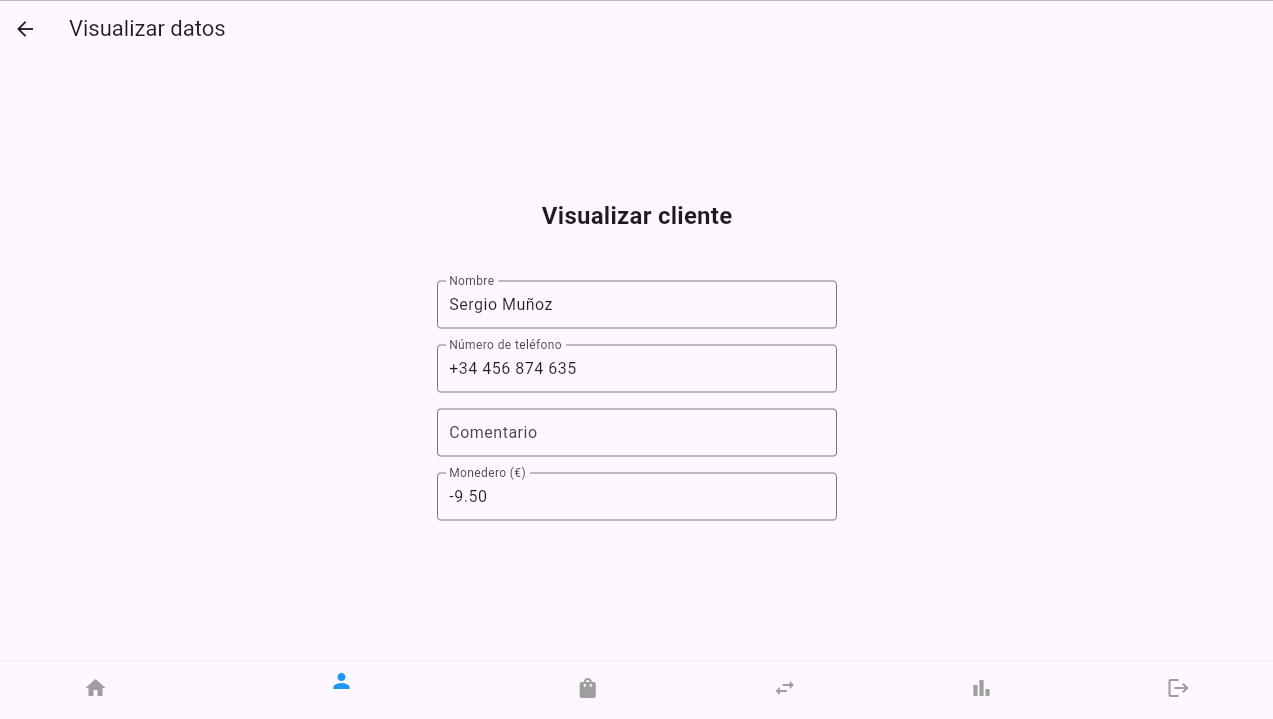
\includegraphics[width=0.7\textwidth]{imagenes/PrimeraIteracion/detallesCliente.png}
	\caption{Interfaz de usuario de la pantalla de visualizar datos de un cliente.}
	\label{fig:appDetallesCliente}
\end{figure}

\subsubsection{Pantalla de visualizar las categorías de artículos}

Se pueden añadir tantas categorías como el usuario crea conveniente para poder organizar los productos de su tienda a su gusto. 

\begin{figure}[H]
	\centering
	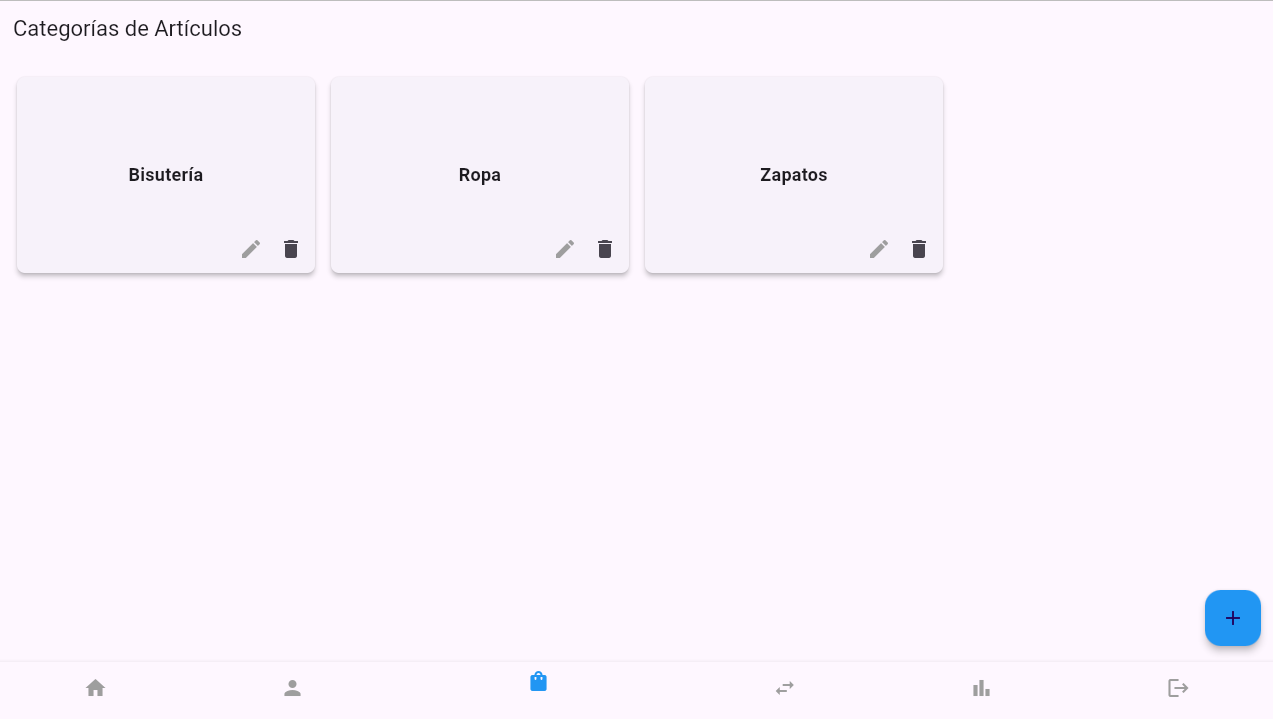
\includegraphics[width=0.7\textwidth]{imagenes/PrimeraIteracion/visualizarCategorias.png}
	\caption{Interfaz de usuario de la pantalla de visualizar las categorías.}
	\label{fig:appCategoriasArticulos}
\end{figure}

\subsubsection{Pantalla de añadir una nueva categoría de artículos}

Cuando se añade una nueva categoría, se deberá de especificar el nombre de dicha categoría y se podrán desmarcar los campos que no sean necesarios para esa categoría. Al marcar o desmarcar un campo, se cambia la visibilidad de este en todos los artículos que estén contenidos en esa categoría. Así se evita incluir campos que no tengan relevancia en ciertas categorías. 

\begin{figure}[H]
	\centering
	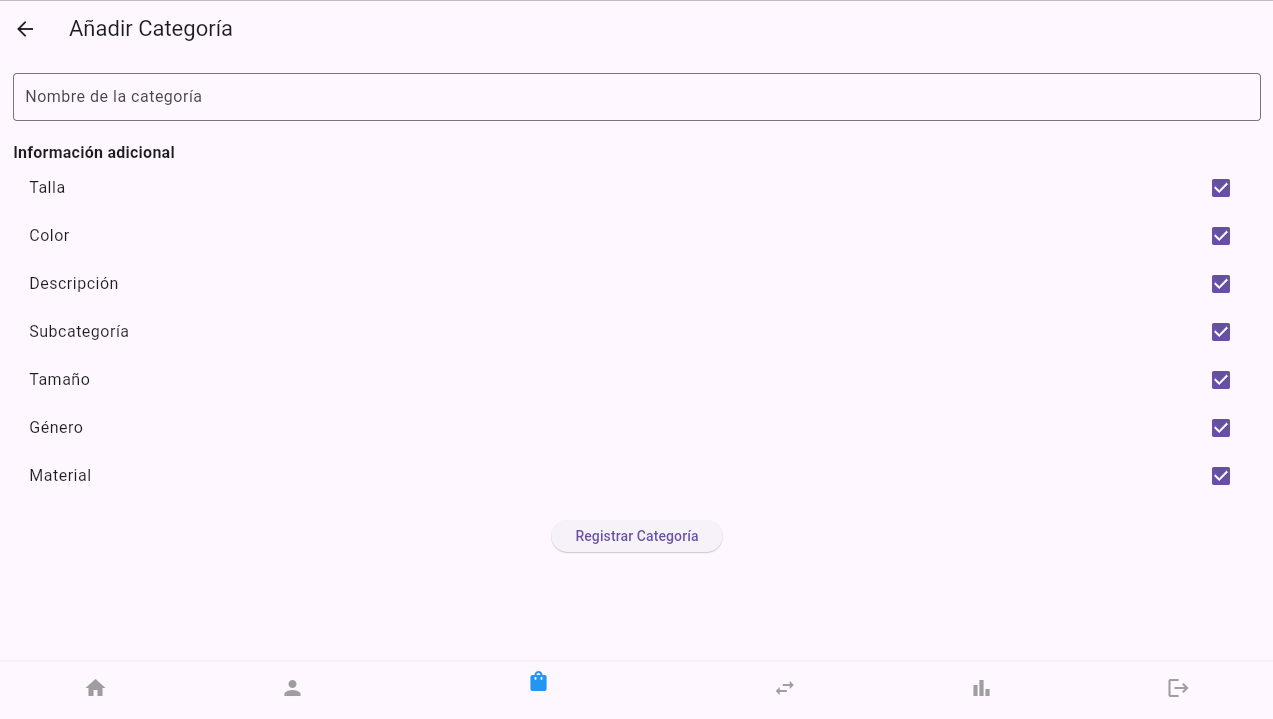
\includegraphics[width=0.7\textwidth]{imagenes/PrimeraIteracion/nuevaCategoria.png}
	\caption{Interfaz de usuario de la pantalla de añadir nueva categoría.}
	\label{fig:appNuevaCategoria}
\end{figure}

\subsubsection{Pantalla de editar una categoría existente}

\begin{figure}[H]
	\centering
	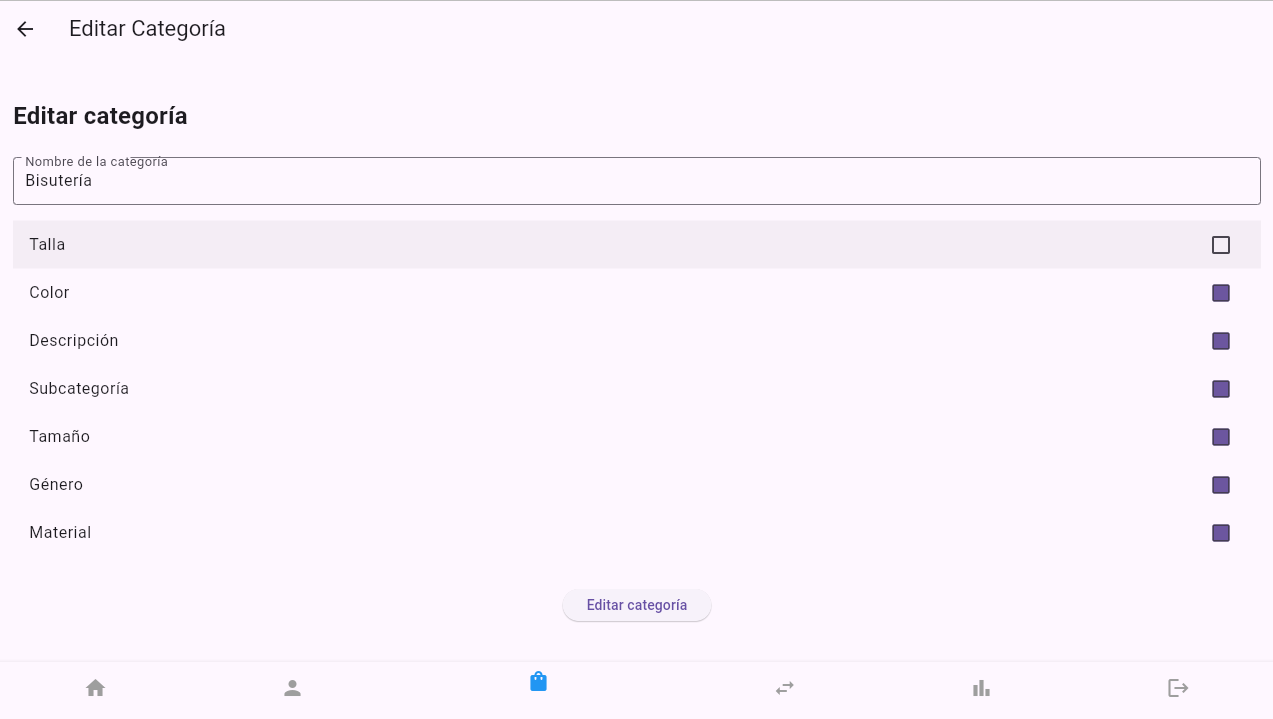
\includegraphics[width=0.7\textwidth]{imagenes/PrimeraIteracion/editarCategoria.png}
	\caption{Interfaz de usuario de la pantalla de editar una categoría.}
	\label{fig:appEditarCategoria}
\end{figure}

\subsubsection{Pantalla de visualizar los artículos de una categoría}

En esta pantalla se ven todos los artículos de una determinada categoría. Se puede buscar por nombre o filtrar por subcategoría. 

\begin{figure}[H]
	\centering
	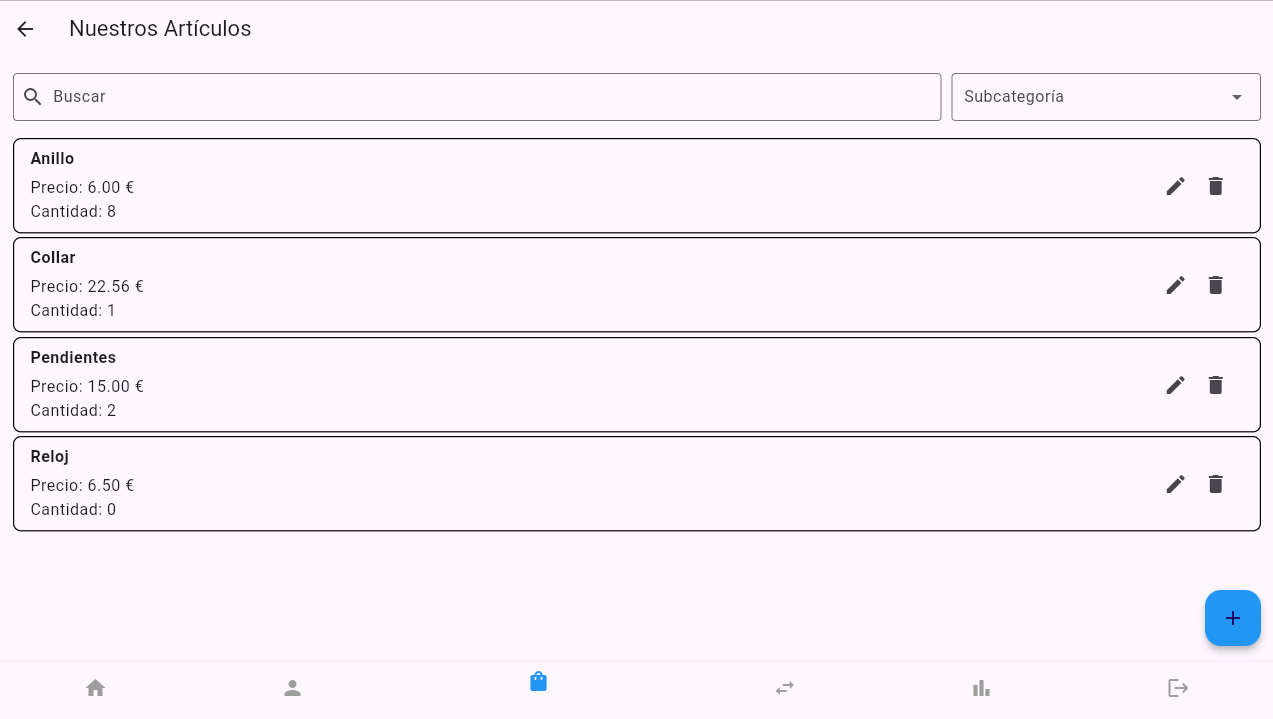
\includegraphics[width=0.7\textwidth]{imagenes/PrimeraIteracion/visualizarArticulos.png}
	\caption{Interfaz de usuario de la pantalla de visualizar artículos.}
	\label{fig:appVisualizarArticulos}
\end{figure}

\subsubsection{Pantalla de añadir un nuevo artículo a una categoría}

\begin{figure}[H]
	\centering
	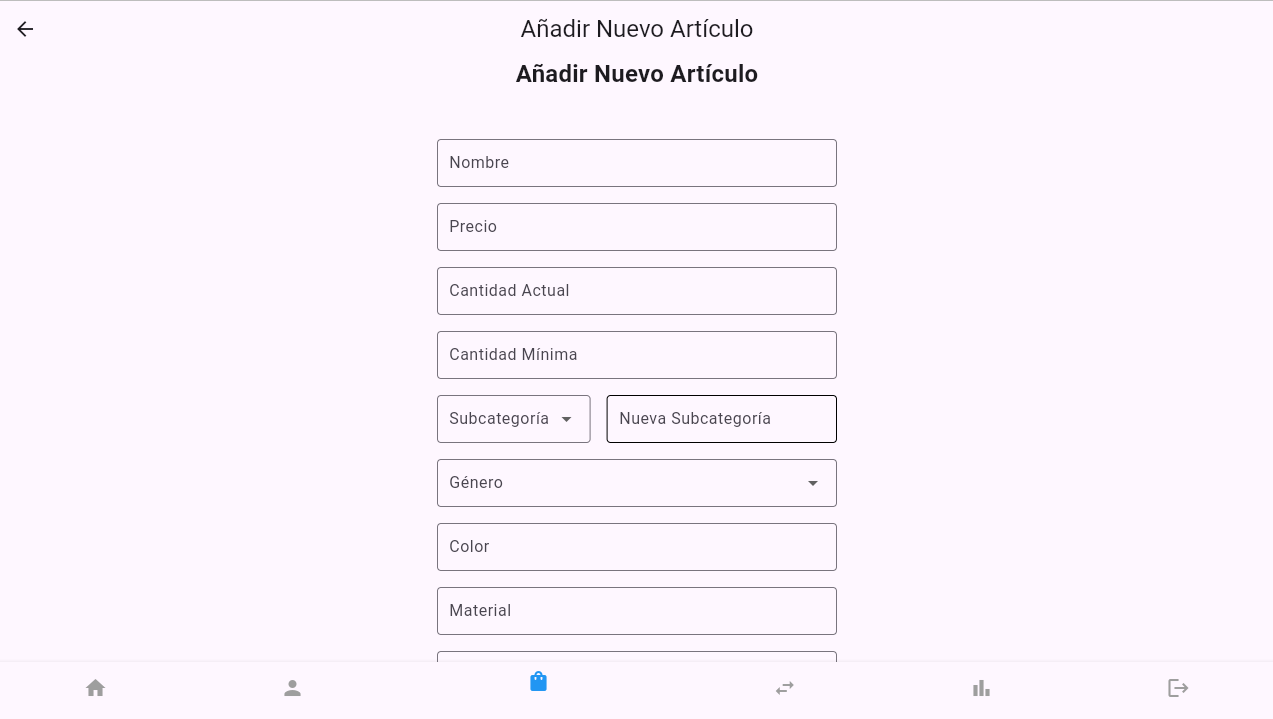
\includegraphics[width=0.7\textwidth]{imagenes/PrimeraIteracion/nuevoArticulo.png}
	\caption{Interfaz de usuario de la pantalla de añadir un nuevo artículo.}
	\label{fig:appNuevoArticulo}
\end{figure}

\subsubsection{Pantalla de editar un artículo existente de una categoría}

\begin{figure}[H]
	\centering
	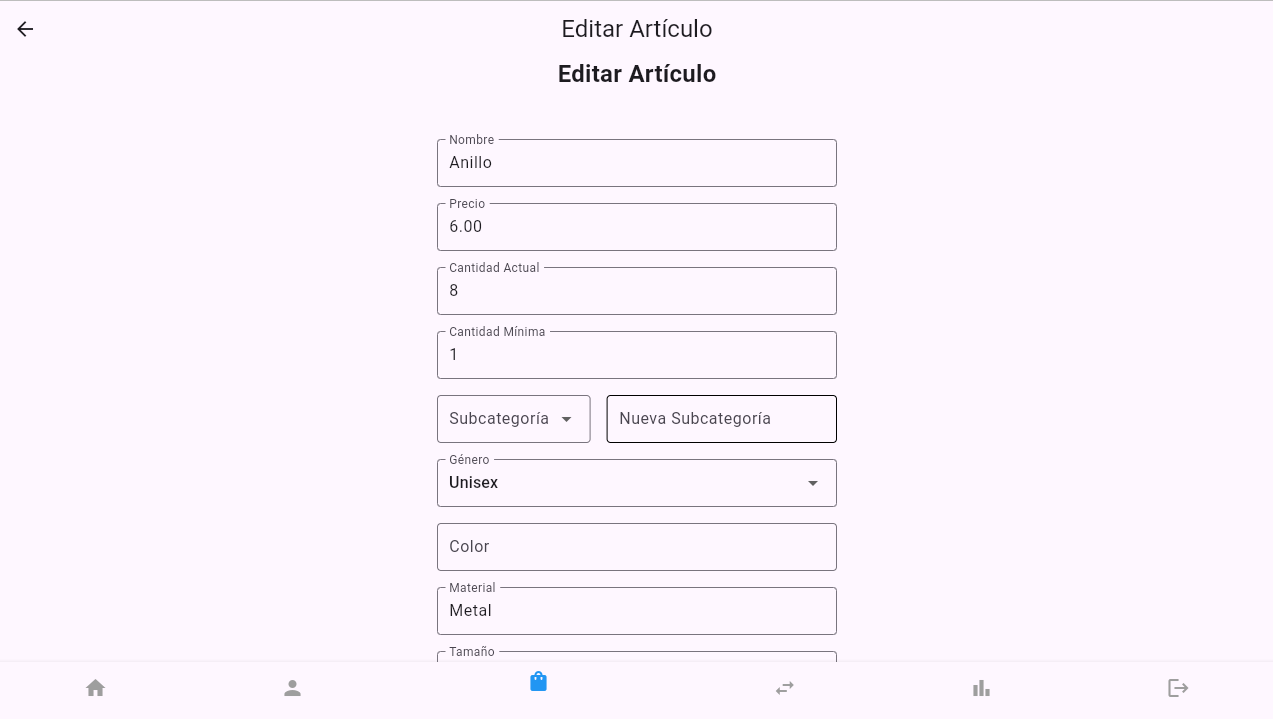
\includegraphics[width=0.7\textwidth]{imagenes/PrimeraIteracion/editarArticulo.png}
	\caption{Interfaz de usuario de la pantalla de editar un artículo existente.}
	\label{fig:appEditarArticulo}
\end{figure}


\subsection{Revisión de la iteración}

\subsubsection{Autenticacion}

El cliente probó el sistema de autenticación y le pareció correcto. 

\subsubsection{Gestión de clientes}

El cliente probó este conjunto de pantallas que gestionan los clientes de la tienda. Pidió una mejora en la accesibilidad en la pantalla de visualizado de clientes. No diferenciar únicamente cuando un cliente debe con un sistema de colores (verde/rojo), añadir también un icono que lo represente. El resto de funcionalidades estaban correctas. 

\subsubsection{Gestión de artículos}

El cliente probó este conjunto de pantallas que gestionan los artículos de la tienda y decidió que no se estaban organizando de forma correcta. Las categorías estaban bien, pero a la hora de añadir nuevos artículos, el formulario debería de permitir añadir varias tallas, no únicamente una. Además, por cada talla, se debería de gestionar la cantidad actual, cantidad mínima y color. 

El resto de funcionalidades estaban bien.  


\subsection{Plan para la próxima iteración}

Para la próxima iteración se propone:

\begin{itemize}
	\item Implementar las mejoras señaladas por el cliente.
	\item Implementar la pantalla de la lista de renovación de artículos.
	\item Implementar las pantallas de gestión de movimientos.
\end{itemize}

\section{Segunda iteración}

\section{Tercera iteración}